% переструктурировать и перерабоать
% мало подробностей: больше -- лучше
% больше методов построения маршрутов
% псевдокод!
% результаты работы перекачуют в другую главу
\chapter{Методы построения маршрутов}
% постановка задачи
Сформулируем постановку задачи формирования маршрутов. Пусть заданы \( N_s \) – число узлов (остановочных 
пунктов), \( N_r \) – число маршрутов. Требуется построить \( N_r \) последовательностей узлов, при которых 
целевая функция качества маршрутной сети будет принимать максимальное значение. 

Задача тесно связана с задачей маршрутизацией <<из пункта А в пункт Б>>, но имеет некоторые отличия. 
Во-первых, в типовой задаче маршрутизации целевая функция – это время поездки от начала до конца маршрута, 
которое необходимо минимизировать. В случае с построением сети маршрутов общественного транспорта целевая 
функция -- интегральная, учитывающая средние показатели времени пешего хода до остановки, длины пути, 
количества пересадок, и пр. [16,17]. Во-вторых, в типовой задаче маршрутизации для движения выбираются 
любые промежуточные точки, сокращающие маршрут, тогда как в рассматриваемой задаче промежуточные точки 
расположены там же, где и центры кластеров.
% ---
Предлагается две стратегии генерации исходной сети маршрутов общественного транспорта. Первая предполагает 
генерацию одного <<длинного>> маршрута, обходящего все исходные узлы. Далее осуществляется разрез маршрута 
на \( N_r \) маршрутов и осуществляется модификация сети в соответствии с эволюционным алгоритмом. Вторая 
стратегия: формирование начальной сети, число маршрутов в которой соответствует заданному значению \( N_r \) 
и применение эволюционных алгоритмов для поиска сети маршрутов с минимальной длиной.
% ---

\section{Жадный алгоритм}
\subsection{Общее описание}
Поглощающий алгоритм (<<жадный алгоритм>>) -- тип алгоритмов оптимизации, которые на каждом шаге выбирают 
локально оптимальную альтернативу -- ту, которая приносит на этом шаге максимальную выгоду. Работают быстро, 
но обычно дают глобально неоптимальное решение, так как пропускают случай, когда лучше на данном шаге 
выбрать не самую лучшую альтернативу, но затем на следующем шаге получить значительный выигрыш.

Входные данные: полносвязанный граф, в котором вершины заданы географическими координатами и количеством 
точек отправления или назначения в кластере, а рёбрам предписаны веса, которые означают потребность в 
перевозке пассажиров между кластерами. Это может быть, например, количество необходимых перевозок в час в то 
или иное время суток (например, в часы пик или же наоборот в спокойное время).

В результате кластеризации исходных данных на предыдущем этапе получен полносвязанный граф, вершины 
которого -- центры кластеров (заданы географическими координатами и количеством точек отправления или 
назначения в кластере). Веса рёбер -- потребность в перевозке пассажиров между кластерами. 

\subsection{Схематическое представление}
Последовательность работы алгоритма описывается следующими шагами:
\begin{enumerate}
    \item 1) определяем ребро графа с максимальной потребностью в транспорте;
    \item 2) выбираем из двух вершин, которые это ребро соединяет, одну, с максимальным количеством 
        пассажиров в ней;
    \item 3) делаем первый шаг из этой вершины в другую, выбирая то ребро, которое имеет максимальную 
        потребность;
    \item 4) из этой вершины делаем шаг в следующую, тоже выбирая ребро с максимальной потребностью:
    \begin{itemize}
        \item если два ребра имеют одинаковую пропускную способность, то выбираем любое;
        \item если ребро имеется в списке, то выбираем следующее по пропускной способности;
    \end{itemize}
    \item 5) строим до тех пор, пока длина маршрута не превысит пороговое значение;
    \item 6) переходим к пункту 1, выбрав следующее по пропускной способности ребро.
\end{enumerate}

\subsection{Результат работы}
Пример работы алгоритма приведен на \ref{img:greedy-01}.
\begin{enumerate}
    \item 1. Выбираем ребро с потребностью перевозки 300.
    \item 2. Выбираем кластер с количеством точек 500.
    \item 3. Первый шаг: начинаем маршрут с ребра 300.
    \item 4. Второй шаг: выбираем ребро 200.
    \item 5. Третий шаг: выбираем ребро 100.
\end{enumerate}

\begin{figure}[h!]
    \centering
    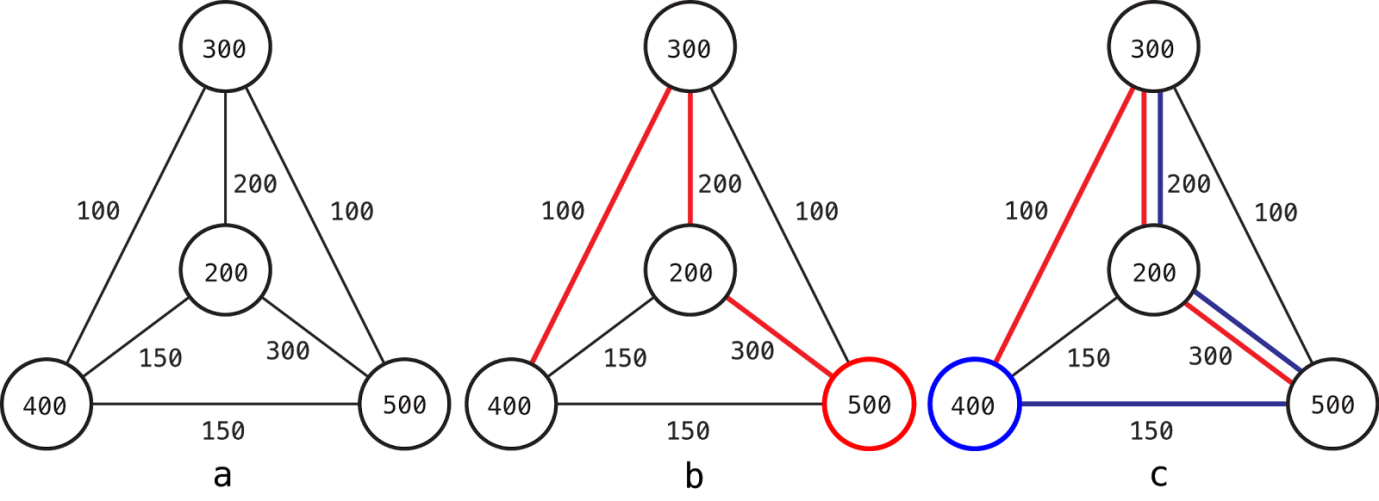
\includegraphics[width=0.47\textwidth]{greedy-01}
    \caption{Пример реализации алгоритма a – исходный граф;
        b – первый построенный маршрут (вершина начала пути выделена красным);
        c – второй построенный маршрут (вершина начала пути выделена синим)}
   \label{img:greedy-01}
\end{figure}
% -----
% нарисовать/найти pdf-ку для жадного алгоритма
% -----

% \subsection{Подробное описание}

\section{Алгоритм минимального увеличения длины}
% ---
\subsection{Общее описание}

Формирование начальной сети маршрутов, используя принцип <<минимального>> увеличения длины маршрута при 
включении нового пункта. Идея алгоритма заключается в итеративном добавлении в существующие маршруты узлы, 
минимально увеличивающие длину исходных маршрутов. 

На вход алгоритма подаються: \( N_r \) -- число маршрутов в сети, \( N_c \) –- число узлов 
(центров кластеров), \( C_t \) – множество терминальных узлов (определенных посредством построения 
окружности, содержащей все узлы), \( C_{nt} \) – множество нетерминальных узлов (сумма элементов множества 
терминальных и нетерминальных узлов равна числу центров кластера), матрица длин размером 
\( ||{C_{nt}} + {C_{t}}|| \times ||{C_{nt}} + {C_{t}}|| \). Заметим, что \( C_t + C_{nt} = n_c \)

Выходом алгоритма является транспортная сеть \( RN \), содержащие непересекающие множество узлов, 
\( r_{i} = [p_{1}^{(i)}, \dots, p_{k}^{(i)}] \), где \( i = 1, \dots, n_r \). 

\subsubsection{Идея метода}
Данный алгоритм содержит следующие шаги
\begin{enumerate}
    \item[Шаг 1] Создать \( n_r \) прямых маршрутов, содержащих пары противоложных терминальных 
        узлов из \( C_t \) и добавить их в \( R_i \)
    \item[Шаг 2] Для каждого \( i \)-го маршрута из сети \( R_i \) выполнить:
    \begin{enumerate}
        \item[2.1] Выбрать \( i \)-тый маршрут из \( R_i \) и разделить его на пары и добавить их в \( PN \);
        \item[2.2] Найти такой узел \( C_t \), который минимально увеличивает длину маршрута из \( PN \) и 
            добавить новый маршрут, включающий данный узел, в \( RC \);
        \item[2.3] Составить \( ||RC|| \) вариантов новых маршрутов: один взятый из сети \( RC \), другой 
            из сети \( PN^{(R_{i})} \) и составить список кандидатов на замену в \( RCC \);
        \item[2.4] Оценить длины маршрутов в \( RCC \) и выбрать маршрут \( R^{\star}_{i} \) 
            с минимальной длиной;
        \item[2.5] Заменить \( R_{i} \) на $R^{\star}_{i}$ в маршрутной сети \( RN \);
        \item[2.6] Удалить узел \( c_{j} \) из \( C_{nt} \) добавленный в \( R^{\star}_{i} \). 
    \end{enumerate}
    \item[Шаг 3] Если \( C_t \) не пустое, перейти на шаг 2, иначе закончить построение.
\end{enumerate}

\subsection{Схематическое представление}
Псевдокод алгоритма представлен следующей схемой \ref{alg:min-length}.
\begin{algorithm}[ht]
    \caption{Алгоритм построения маршрутной сети}
    \KwData{\( N_r, C_t, C_nt \)}
    \KwResult{\( RN \)}
    \For{\( i=1 \ldots N_r \)}{
        1. Построить \( R_{i} \) прямой маршрут включающий пару терминальных кластеров из \( C_t \)\;
        2. Добавить \( R_{i} \) в \( RN \);\
    }
    \While{\( C_{nt} \) не пусто}{
        \For{\( i=1 \ldots N_r \)}{
            1. Выбрать \( R_{i} \) из \( RN \), \( R_{i} = [n_1, n_2, \ldots n_{R}] \)\;
            2. Разделить \( R_{i} \) на пары
                \( PN^{(R_{i})} = [[n_1, n_2] , [n_2, n_3], \ldots, [n_{R-1}, n_{R}]] \)\;
            3. Инициализировать список \( RC \)\;
            4. \For{пары \( [n_x, n_y] \) из \( PN^{(R_{i})} \)}{
                4.1 Найти узел минимально увеличивающий маршрут \( [n_x, n_y] \), т.е. найти узел \( c_j \)
                    из \( C_{nt} \), где \( j = argmin (|len(n_x, n_y)  - (len(n_x, c_j, n_y))|) \)\;
                4.2 Добавить \( [n_x, c_j, n_y] \) в \( RC \)\;
            }
            5. Составить \( ||RC|| \) вариантов новых маршрутов: один взятый из сети \( RC \), другой 
                из сети \( PN^{(R_{i})} \) и составить список кандидатов на замену в \( RCC \)\;
            6. Посчитать длины маршрутов в \( RCC \) и выбрать маршрут \( R^{\star}_{i} \) с 
                минимальной длиной\;
            7. Заменить \( R_{i} \) на \( R^{\star}_{i} \) в \( {RN} \)\;
            8. Удалить узел \( c_{j} \) входящий в \( R^{\star}_{i} \) из \( C_{nt} \)\;
        }
    }
    \label{alg:min-length}
\end{algorithm}

\subsection{Explanation}
Let consider an explanation of the proposed algorithm by simple example. Given terminal nodes indicated as 
\( A, A', B, B' \) (\( C_t \)) and nonterminal nodes indicated as \( C, D, E, F \) (\( C_{nt} \). Assume 
the number of routes is \( n_r = 2 \). So the results are two routes covers all terminal and nonterminal 
nodes.

The first step is to define direct routes which include only terminal nodes. We agreed to add into initial 
route opposite nodes which are located opposite one another. So the route list contains two routes 
\( R_i = [AA', BB'] \). Figure \ref{fig:route_first} shows the initial direct routes.

\begin{figure}[ht!]
    \centering
    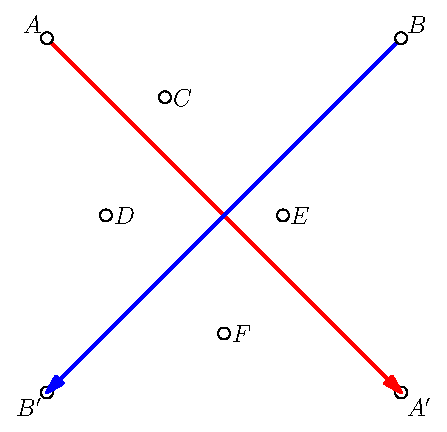
\includegraphics[width=0.47\textwidth]{route01}
    \caption{Initial routes network including \( n_r \) direct routes with terminal nodes.}
    \label{fig:route_first}
\end{figure}

Next, we choose the next route from the list \( R_i \) and divide the route in half. As we have two nodes 
in the route, there is the only one route \( PN = [AA'] \).

Next we compose a new set of routes by adding the new node as the midpoint in existed routes from \( PN \). 
In this case, we have \( ACA', ADA', AEA', AFA' \). 

Getting these four new routes we calculate the length each of them and selects the route with minimal 
length (in our case of \( ACA' \)). Add \( ACA' \) in the routes list \( RC = [ACA'] \).

Next, we compose all variants of routes from lists \( RC \) and \( PN \). In this case we have only one 
route \( ACA' \), so we add it to the list \( R^{\star}_{i} \). Node \( C \) is removed from the list 
\( C_nt \). The same actions for the second route from initial list and get new route \( BEB’ \). 
Figure \ref{fig:route_second} represents the routes network after first iteration. 

\begin{figure}[ht!]
    \centering
    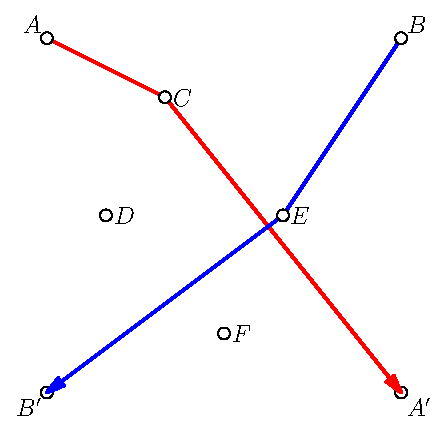
\includegraphics[width=0.47\textwidth]{route02}
    \caption{Routes network after the first iteration.}
    \label{fig:route_second}
\end{figure}

Starting the second iteration we have a list of routes \( R_i = [ACA', BEB'] \). Using \( ACA' \) we have 
two pairs \( PN=[AC, CA'] \). 

Sequentially adding every non-terminal node and have \( ADC, AFC, CDA', CFA' \). The shortest route is 
\( CDA' \). 

Compose different variants from \( CDA' \) and \( AC \), \( CA' \) and get \( ACDA' \). Add new route 
into \( R^{\star}_i \) and remove \( D \) from \( C_nt \).

Similarly, for the second route from \( R_i \) we get \( BEFB' \).

As \( C_nt \) contain no more nodes (empty set) the algorithm is terminated. 

Figure \ref{fig:route_third} represents the final result.

\begin{figure}[ht!]
    \centering
    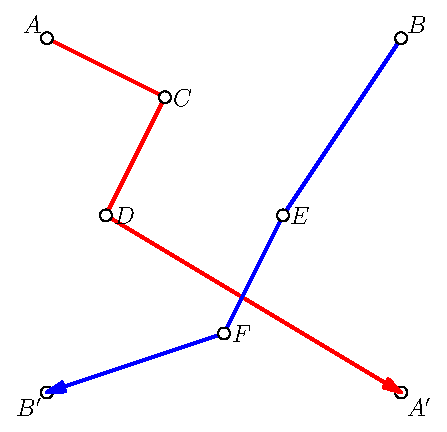
\includegraphics[width=0.47\textwidth]{route03}
    \caption{Final routes network.}
    \label{fig:route_third}
\end{figure}

\subsection{Using of convex hull algorithm}
We used the simple idea to find terminal nodes in initial direct routes (step 1). Terminal nodes are found 
based on  the idea of convex hull algorithm. 

For all given nodes, the convex hull is created. It helps to draw a circle circumscribed about the convex 
hull. Since we have a number of routes as an initial parameter, we define \( 2\cdot N_r \) equally-spaced 
nodes on the circle. Opposite pair of nodes is a quasi-origin/destination nodes in the routes. To define 
the real origin/destination, we found the nearest node to quasi-nodes.

\subsection{Результаты работы}
Алгоритм был апробирован на различных тестовых данных для различных значений числа маршрутов. 
Результат работы алгоритма представлен на \ref{img:min-length-01}.
\begin{figure}[h!]
    \centering
    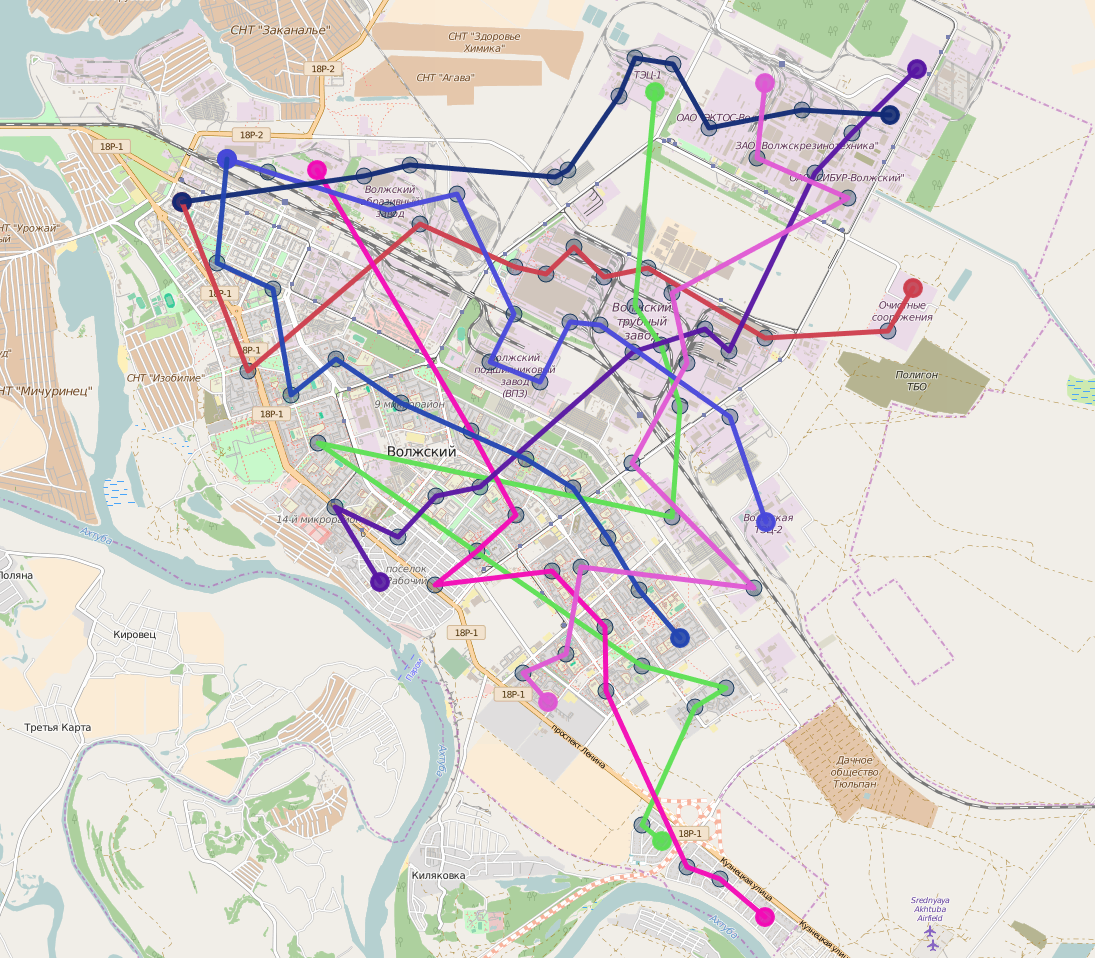
\includegraphics[width=0.47\textwidth]{minimal-01}
    \caption{Визуализация результата работы алгоритма формирования начальной сети маршрутов, 
        использующий принцип <<минимального>> увеличения длины маршрута при включении нового пункта.}
   \label{img:min-length-01}
\end{figure}

% \subsection{Подробное описание}

\section{Алгоритм модификации начальной сети маршрутов}
% ---------------
% 3 метод -- WIP
% ---------------
\emph{Модификация начального варианта сети маршрутов общественного транспорта с целью минимизации функции 
затрат и генерация вариантов альтернатив сетей}
\subsection{Общее описание}
Модификация начального варианта сети маршрутов общественного транспорта осуществляется с использованием идеи 
итерационного эволюционного преобразования исходного маршрута. Предлагается эволюционный алгоритм, 
использующий операции мутации и кроссовера для оптимизации длины сети маршрутов [19].

\subsection{Идея метода}
Эволюционный алгоритм представлен следующей последовательностью шагов. 
\begin{enumerate}
    \item[1.] Если выбрана стратегия формирования единственного начального маршрута, то 
    \begin{enumerate}
        \item[1.1.] Сформировать единственный маршрут жадным алгоритмом.
        \item[1.2.] Разрезать маршрут на \( k \) маршрутов (где \( k \) -- изначально заданное число 
            маршрутов).
    \end{enumerate}
    \item[2.] Если выбрана стратегия формирования начальной сети, то перейти на шаг 3.
    \item[3.] Оценить качество сети маршрутов (с использованием критериев качества, например длины 
        маршрутной сети).
    \item[4.] Применить операцию кроссовера и мутации для получения новой генерации транспортной сети [19].
    \begin{enumerate}
        \item[4.1.] Оценить качество новой сети маршрутов.
        \item[4.2.] Если новая популяция лучше предыдущей, сохранить ее.
        \item[4.3.] Если новая популяция хуже предыдущей, отклонить. 
    \end{enumerate}
    \item[5.] Повторить, пока не выполняется условие останова.
\end{enumerate}

\subsection{Схематическое представление}
\subsection{Результаты работы}

% \subsection{Подробное описание}
% ---

\section{Заключение}